
\chapter{基于SSA的函数式编译器概览} \label{sec:overview}

本文构建了一个从函数式程序到LLVM IR的编译器,并完成了对其核心编译步骤的形式化验证。
我们在Coq定理证明工具中完成了编译算法和形式化验证相关定理证明的实现。

我们选取PCF(Programming Computable Functions)语言作为该函数式编译器的源语言,因为它是函数式编程语言的核心,
被广泛应用于关于函数式语言的研究~\cite{plotkin1977lcf,ABRAMSKY2000409}。
尽管PCF是一种小规模的语言,但它是图灵完备的,即所有可计算的函数都可以表示为PCF程序。
把它作为该编译框架的源语言,不会使算法和验证过于复杂而无法完成,也能够说明关键问题。

在本章中,我们主要是从高层次的角度介绍了这个编译器原型,省略了转换算法细节和定理证明的详细信息。
该编译器读取PCF程序,并经过图~\ref{overview}中所示的几个编译步骤生成LLVM IR程序。
对于核心编译过程CPS转换及CPS到SSA的转换,我们对它们的正确性进行了形式化验证。
遵循第~\ref{sec:compcertbackend}节中所介绍的CompCert后端的验证框架,
我们通过建立源程序和目标程序之间的后向模拟完成了形式化验证。
本文中使用$\approx $符号表示源程序和目标程序的语义保存性质。
PCF、CPS和SSA的程序分别表示为$t_{pcf}$、$t_{cps}$和$t_{ssa}$。
通过对$t_{pcf}\approx t_{cps}$和$t_{cps}\approx t_{ssa}$的形式化证明,可以组合推导出$t_{pcf}\approx t_{ssa}$。

\begin{figure}[htbp]
    \centering
    \vspace{2ex}
    \includegraphics[width=0.8\linewidth]{figures/overview.pdf}
    \caption{PCF到LLVM编译链概览}\label{overview}
\end{figure}

\section{读入PCF文本}

首先使用PCF语法分析器(Parser)将文本形式的PCF程序提取为Coq中结构化的PCF抽象语法树。
为了分析文本信息从而提取PCF程序,我们需要先对文本进行逐词划分,然后按照语法规则组装起来。
具体来说,对于文本形式的PCF程序,
我们首先用词法分析器(Lexical Parser)将其解析为标记流(Tokens)。
随后,使用语法分析器(Syntax Parser)分析该标记流,生成Coq中直接风格PCF程序项的抽象语法树。

词法分析器和语法分析器在OCaml中实现,是利用词法和语法解析规则及对应操作生成的函数。
具体实现方法将在第~\ref{sec:pcfparser}节中介绍。
得到PCF源程序的抽象语法树后,我们就可以开始对其进行编译了。

\section{CPS转换}

如第\ref{sec:background}节中所言,函数式编程语言的编译器通常会将
直接风格的函数式程序转换为CPS形式,以获得显式的控制流。
经过了上一步,我们已经得到了PCF程序的抽象语法树,但它是直接风格的程序。
所以接下来需要使用CPS转换将其编译为CPS风格的程序。

将直接风格的PCF程序转换为CPS形式的算法$\mathcal{F}$
主要由当前代码项和当前项被规约为某个值后要处理的下一个项决定。
我们使用一个特殊的顶层延续变量,把它应用到CPS程序的返回值上,即用来传递整个代码项的值。
另外,我们为直接风格及CPS形式的PCF语言分别定义了小步操作语义,并证明了CPS转换的前向模拟性质。
关于该CPS转换算法的设计及其正确性验证的详细信息将在第\ref{sec:cpstrans}节和
第\ref{sec:cpsforward}节中进行进一步讨论。

\section{从CPS到SSA}

该编译链中最关键的部分是从CPS风格的函数式程序到目标SSA程序的转换及验证。
这一编译步骤的源程序就是经过了CPS转换的PCF程序。
该转换过程的目标SSA语言是LLVM IR的简化版本,保留了其最基本的结构和程序语句。
虽然CPS是函数式语言,而SSA是命令式语言,它们的程序结构之间有一定的对应关系。
我们在设计转换算法时,主要的根据就是CPS程序与SSA程序结构上的对应关系。
通过该编译过程,输入的CPS程序项将被转换为一个包含主函数的SSA程序。
此步转换是一个递归的过程,它不断将最外层的CPS程序结构转换为SSA组件,
并将这些新的组件放入已有SSA程序的特定位置。当CPS程序最里层的结构都已被处理完毕,
SSA程序就是转换完成的结果了。在这个过程中,SSA程序从一个空的主函数开始,
一步步添加新的指令,基本代码块以及函数等组件,最终形成了编译后的完整SSA程序。

同样的,我们为这种SSA语言定义了小步操作语义,并证明了从CPS到SSA转换的前向模拟。
完成这一步证明后,我们将这一步前向模拟与CPS转换的前向模拟组合起来,
并证明SSA程序的确定性,从而完成从源程序到SSA程序后向模拟的证明。
在第\ref{sec:cpsssatrans}节中将详细介绍该转换算法的设计和细节。
第\ref{sec:cpsssaforward}节中将进行CPS到SSA转换算法的形式化验证,
并通过运行一个示例程序展示前向模拟的每一个关键步骤。

\section{从SSA到LLVM IR}

上一步中得到的SSA程序被转换为Vellvm中的抽象语法树,然后转换为LLVM IR程序文本。
在该编译链中,我们使用了经过验证的LLVM基础设施Vellvm~\cite{zakowski2021modular}。
利用其在Coq实现的LLVM IR的抽象语法树,我们可以进一步输出最终的LLVM IR程序。

由于我们使用的SSA语言是LLVM IR的简化版本,它保留了LLVM IR程序的基本结构,
可以方便地编译到Vellvm中的抽象语法树。这种SSA语言省略了LLVM IR中的大部分参数。
例如,函数定义在LLVM中非常复杂,有很多可选的参数,而本文中的SSA语言只保留了函数定义中必须指定的内容。
LLVM中的表达式类型多种多样,其中整数包括多种宽度的i16、i32等,
而本文的SSA语言简化为没有明确指定类型的无限宽自然数。
该编译过程的主要工作其实就是为这些被省略的参数选取正确的默认值。

\section{核心编译步骤的正确性验证}

构建该编译器的关键工作是从CPS到SSA的转换与验证。
由于函数式程序的CPS转换是函数式编译器中常用的编译过程,
我们也为CPS转换完成了形式化验证。所以,最终该编译器中经验证的
部分是从直接风格PCF到SSA的转换。我们证明了该核心编译过程的语义保存性质。
在对核心编译步骤进行形式化验证时,我们采用的是基于模拟的验证技术。
本文第~\ref{sec:compcertbackend}节中对CompCert提供的形式化验证框架进行了介绍。
我们将这样的理论和框架应用在PCF到SSA的编译过程中,证明了核心编译步骤的正确性。

本文的形式化验证针对的是安全的源程序,即输入的PCF程序要么终止返回结果值、要么发散,不会出错。
并且,PCF程序不会卡在一个非终止的状态下无法进行下一步转换。

利用程序语言的小步操作语义,我们分别为CPS转换和CPS到SSA的转换证明了前向模拟性质。
对于CPS转换,直接风格的PCF程序经过转换算法$\mathcal{F}$转换为CPS形式的程序。
对于CPS到SSA的转换,CPS经过转换算法$\mathcal{G}$转换为SSA程序,即经简化的LLVM IR。
如图~\ref{extracts}所示,我们分别为直接风格PCF语言,CPS语言和SSA语言定义了小步操作语义,
即程序状态之间的最小转换规则。
对于这两步转换,我们分别用目标程序的行为去模拟源程序的每一小步行为,从而分别证明了
两步转换的前向模拟性质。我们将两步编译的前向模拟组合起来,就得到了PCF程序到SSA程序整体
编译过程的前向模拟性质。
接着,我们证明目标SSA语言具有确定性,并结合已经证明的前向模拟性质,
得到PCF到SSA转换的后向模拟,即说明了该转换算法的正确性。

\begin{figure}[htbp]
    \centering
    \vspace{2ex}
    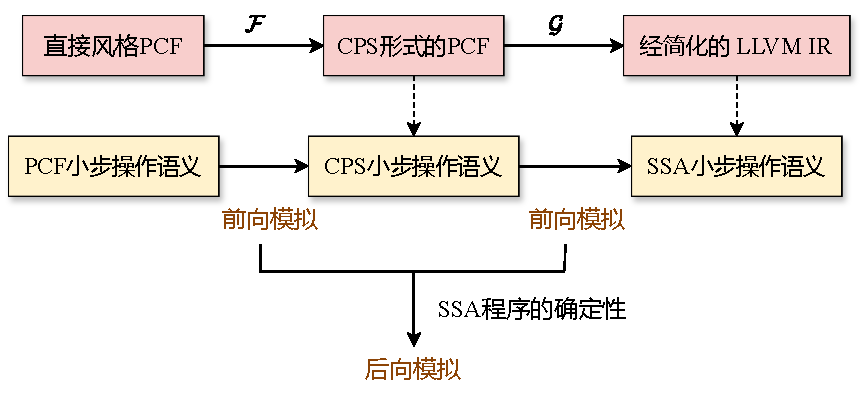
\includegraphics[width=0.8\linewidth]{figures/extracts.drawio.pdf}
    \caption{CPS到SSA基于模拟技术的验证}\label{extracts}
\end{figure}

其中,进行CPS转换时程序内部执行步骤遵循的是多步模拟,如图~\ref{plus}所示。
我们首先定义了直接风格PCF程序状态与CPS程序状态之间的匹配关系$\sim$。
对于PCF源程序$t_{pcf}$,它的初始状态为$S_{pcf1}$。
对于CPS程序$t_{cps}$,它的初始状态为$S_{cps1}$。
PCF源程序经过一步转换,CPS可以在经过一步或多步转换后再次与之状态匹配。
例如,$S_{pcf1}\sim S_{cps1}$,当状态$S_{pcf1}$变为$S_{pcf2}$,
$S_{cps1}$经过一步或多步转换到达状态$S_{cps2}$,使得$S_{pcf2}\sim S_{cps2}$成立。
在CPS转换中,我们不需要考虑无限驻留问题,因为目标程序至少需要走一步。

\begin{figure}[htbp]
    \centering
    \vspace{2ex}
    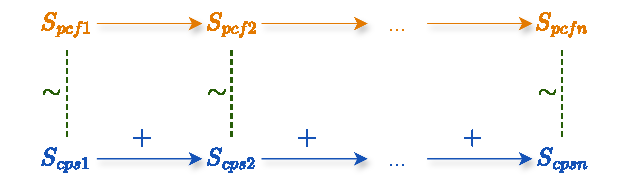
\includegraphics[width=0.75\linewidth]{figures/plus.drawio.pdf}
    \caption{PCF到CPS的多步模拟}\label{plus}
\end{figure}

对于CPS到SSA的转换,程序内部执行步骤遵循的是星形模拟,即如图~\ref{star}所示。
我们同样需要为CPS程序和目标SSA程序定义了程序状态之间的匹配关系$\sim$。
对于SSA程序$t_{ssa}$,它的初始状态为$S_{ssa1}$。
CPS源程序经过一步转换,SSA程序可以在经过零步,一步或多步转换后再次与之状态匹配。
例如,$S_{cps1}\sim S_{ssa1}$,当状态$S_{cps1}$变为$S_{ssa2}$,
$S_{ssa1}$经过零步,一步或多步转换到达状态$S_{ssa2}$,使得$S_{cps2}\sim S_{ssa2}$成立。

\begin{figure}[htbp]
    \centering
    \vspace{2ex}
    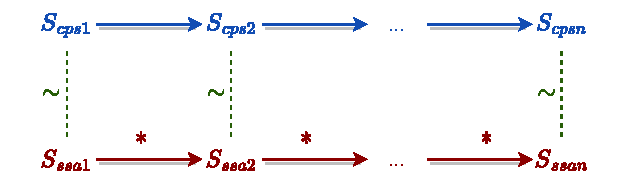
\includegraphics[width=0.75\linewidth]{figures/star.drawio.pdf}
    \caption{CPS到SSA的星型模拟}\label{star}
\end{figure}

正如第~\ref{sec:compcertbackend}节中所言,星型模拟在目标程序进行零步转换仍然匹配时,
可能会出现无限驻留问题。因此,我们为CPS程序定义了度量函数,来防止出现星形模拟中的无限驻留问题。
如图~\ref{stutter}所示,当CPS程序进行一步转换时,SSA程序在原地驻留。
那么,如果CPS程序无限地进行这一步转换,它就会发散,而目标SSA程序始终驻留。
这样一来,源程序和目标程序的行为就不一致了。
所以,为了防止出现这种情况,我们为CPS程序状态定义了递减的度量函数。
度量函数的具体设计及作用将在第~\ref{sec:cpsssaforward}节中详述。

\begin{figure}[htbp]
    \centering
    \vspace{2ex}
    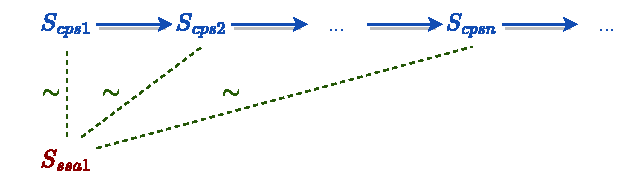
\includegraphics[width=0.75\linewidth]{figures/stutter.drawio.pdf}
    \caption{CPS到SSA可能出现的无限驻留问题}\label{stutter}
\end{figure}

将两步前向模拟组合起来可以得到从PCF源程序到SSA程序的前向模拟。
我们还证明了SSA程序的确定性,即同一个终止的SSA程序返回值是唯一确定的。
利用SSA程序的确定性和前向模拟性质,我们证明了PCF到SSA的后向模拟,
即SSA程序的行为是可接受的PCF程序行为。
这样,我们就验证了从PCF到SSA的核心编译过程的正确性。

完成了这样一个核心编译步骤经验证的基于SSA的PCF语言编译器,我们就用形式化的方法
将CPS与SSA联系在了一起,并为高可靠函数式编译器与主流编译器基础设施的连接提供了基础。
在接下来的两章中,我们将分别详细介绍关键编译步骤的转换算法和其语义保存性质的形式化验证。
该函数式编译器的具体代码实现将在第\ref{ch:implement}章中介绍。